\documentclass[asi]{picINSA}

%\usepackage[latin1]{inputenc}
%\usepackage[T1]{fontenc}
%\usepackage[francais]{babel}
\usepackage{lmodern}
\usepackage{amsmath}
\usepackage{amssymb}
\usepackage{mathrsfs}


% Bout de code pour enlever le ``chapitre'' écrit à chaque fois
\makeatletter
\def\@makechapterhead#1{
  {\parindent \z@ \raggedright \normalfont
    \interlinepenalty\@M
    \Huge\bfseries  \thechapter.\quad #1\par\nobreak
    \vskip 40\p@
  }}
\makeatother
% Enlève les doubles pages blanches inutiles
\let\cleardoublepage\clearpage



\begin{document}

    \titreGeneral{Rapport}
	\sousTitreGeneral{\newline Sujet RPG 1}
	\titreAcronyme{\LARGE IHME}
	\version{1.00}
	\referenceVersion{bibliographie}
	
	\couverture{}

\tableofcontents{}

\chapter{Introduction}
L'objectif de ce projet est, de réaliser un générateur de scénarios pour RPG, et de mettre en place le déroulement de ce scénario. Les différents joueurs pourront être soit humains, soit virtuels. La trame du jeu pourra faire l'objet de re-planiffication si nécessaire, en fonction des actions effectuées par les différents joueurs. L'interface serait très légère de manière à se concentrer sur le scénario et sur le comportement des joueurs virtuels. \\

Dans ce rapport, nous allons commencer par vous présenter les spécifications que nous avons établies à partir de cet énoncé, et dans un second temps la conception à lequelle nous sommes parvenus.


\chapter{Spécifications}
Après réunions et discussions entre les membres du groupe, voici les spécifications auquelles nous sommes parvenues : \\
~\\
\textbf{A faire nécessairement} :
\begin{itemize}
\item Positionnement (PNJ/Objet), méthode de déplacement, gestion de l'inventaire et de l'argent
\item Interaction entre et avec les PNJ (communication)
\item Objectifs/Scénarios/Quête (décomposées en plusieurs étapes, cachées ou explicites)
\item Maître du Jeu (aide du joueur et re-planification du scénario)
\end{itemize}
~\\
\textbf{A faire dans un second temps} :
\begin{itemize}
\item PNJ ayant leurs objectifs et leurs désirs propres
\item Gestion des connaissances (en fonction de l’intelligence)
\item Gestion des distances pour les interactions
\item Lien avec le programme developpé par Quentin BATEUX
\end{itemize}
~\\
\textbf{A faire si possible} :
\begin{itemize}
\item Interaction entre PNJ (communication de l'émotion)
\item Expérience
\item Interaction entre PNJ et path finding et combat (en lien avec ce que fait l'autre groupe RPG)
\end{itemize}
~\\
\textbf{Optionnel} :
\begin{itemize}
\item Interaction évoluées entre PNJ (accointance, amitié, mariage, couple, enfant)
\item Transmission des gènes et des désirs
\item Évolution des objectifs selon des formules de psychologie (formule parabolique de la motivation sur [0;1])
\item Gestion des connaissances "instantanées" sur le monde.
\item Gestion de la respiration
\item Gestion des différents milieux
\item Gestion de la faim et de la soif
\item Gestion des bâtiments
\item Gestion du statut social
\item Tri des objectifs selon la pyramide de Maslow
\end{itemize}


\chapter{Conception}
Nos choix de conception ont été faits en nous basant sur les résultats des synthèses bibliographiques que nous avons faites par groupe de 2. \newline

Une des synthèses concernait l'Intelligence Artificielle dans les jeux vidéos, et après renseignements, nous sommes arrivés à la conclusion que l'utilisation d'un BDI est la solution la plus adaptée au projet. Nous avons donc mis en place un BDI, en l'adaptant à notre projet. \\

L'autre synthèse bibliographique concernait la scénarisation automatique. Nous avons choisi de mettre en place un HTC pour modéliser les actions des personnages. \\

\section{Conception générale}

\subsection{Diagramme de package}
\begin{figure}[!ht]
  \begin{center}
    \includegraphics[width=1\textwidth]{../conception/packages.pdf}
    \caption{Diagramme de packages}	
  \end{center}
\end{figure}



\subsection{Diagramme de classe}
\begin{figure}[!ht]
  \begin{center}
    \includegraphics[width=1\textwidth]{../conception/Conception.pdf}
    \caption{Diagramme de classe}	
  \end{center}
\end{figure}



\section{Interface graphique}
Etant donné la taille du projet, nous avons opté pour une interface graphique simple, fonctionnant en ligne de commande. Nous avons mis en place un affichage du monde par \textit{AsciiArt}, complété eventuellement par d'autres informations écrites. La récupération des actions de l'utilisateur se fait par saisi de mots-clés parmis une liste d'actions possibles.

\subsection{Représentation du monde}
La représentation du monde en \textit{AsciiArt} fonctionne ainsi :
\begin{itemize}
\item chaque case du monde est représenté par un carré de 3 lignes et 3 colonnes, soit 9 symboles.
\item 4 types de terrains sont possibles : herbe, terre, forêt, et montagne. Ils sont représentés par les symboles suivants : \\
\begin{tabular}{| c c c | c c c | c c c | c c c | }
 \hline		
  \multicolumn{3}{|c|}{herbe} & \multicolumn{3}{|c|}{terre} & \multicolumn{3}{|c|}{forêt} & \multicolumn{3}{|c|}{montagne} \\	
\hline
    \verb+"+ & \verb+"+ & \verb+"+ & $\equiv$ & $\equiv$ & $\equiv$ & $\phi$ & $\phi$ & $\phi$ & $\triangle$ & $\triangle$ & $\triangle$ \\
    \verb+"+ & \verb+"+ & \verb+"+ & $\equiv$ & $\equiv$ & $\equiv$ & $\phi$ & $\phi$ & $\phi$ & $\triangle$ & $\triangle$ & $\triangle$ \\
    \verb+"+ & \verb+"+ & \verb+"+ & $\equiv$ & $\equiv$ & $\equiv$ & $\phi$ & $\phi$ & $\phi$ & $\triangle$ & $\triangle$ & $\triangle$ \\
 \hline  
 \end{tabular}
~\\
\item un objet est représenté par un $\blacklozenge$ à droite de la case.
\item un PNJ est représenté par un $\theta$ à gauche de la case.
\item le joueur est représenté par un $\bigoplus$ au centre de la case.
\end{itemize}

\subsubsection{Exemple}
Dans l'exemple ci-dessous, on peut voir un monde de 5 x 5 cases, avec un PNJ dans la case (1,1), un autre dans la case (5, 4), un objet à la case (0, 5), un autre objet sur la case (5, 1) et enfin le joueur sur la case (3, 3).

\begin{figure}[!ht]
  \begin{center}
    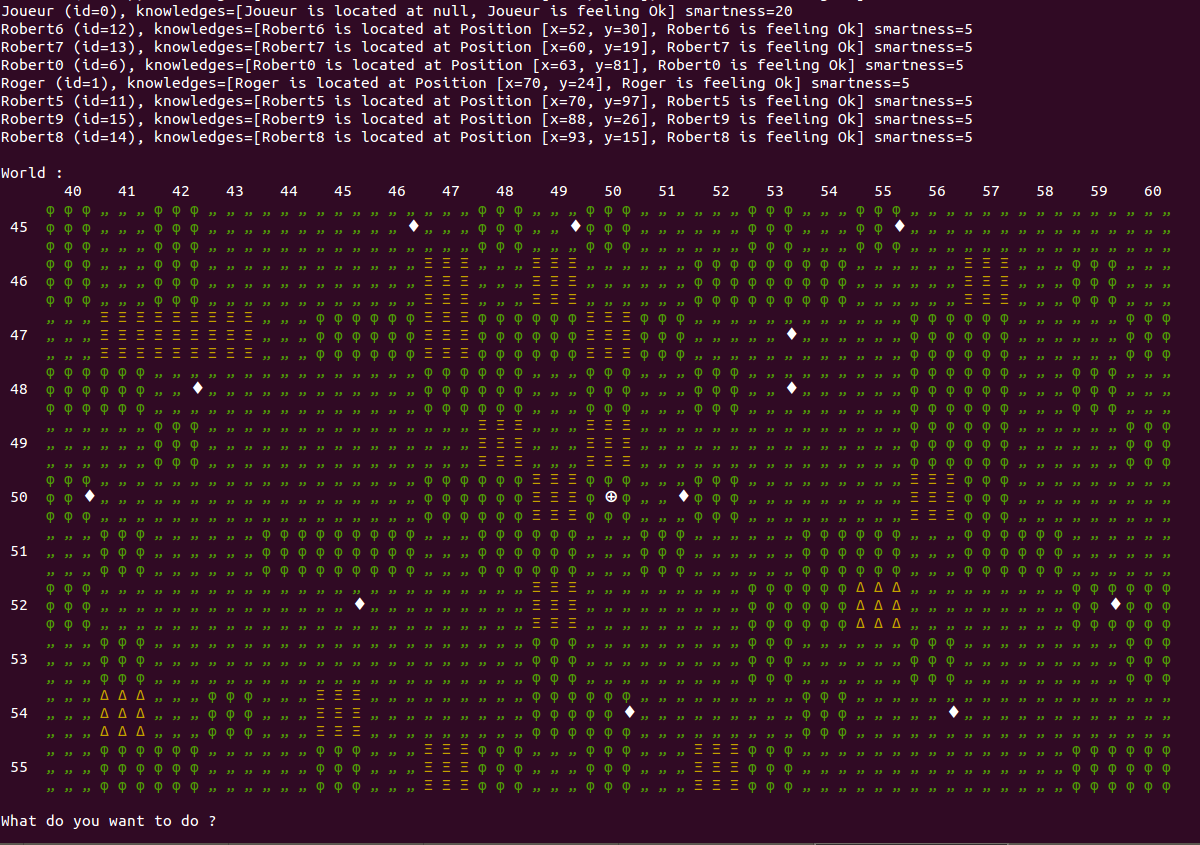
\includegraphics[width=1\textwidth]{images/screenshootWorld01.png}
    \caption{Exemple de la représentation d'un monde de taille 5 x 5 avec 2 PNJ et 2 objets}	
  \end{center}
\end{figure}

\subsection{Interaction du joueur}
Les interactions avec le joueur se font en lui proposant différentes actions et en le laissant choisir par mot-clés, comme dans l'exemple ci-dessous : \\
\begin{figure}[!ht]
  \begin{center}
    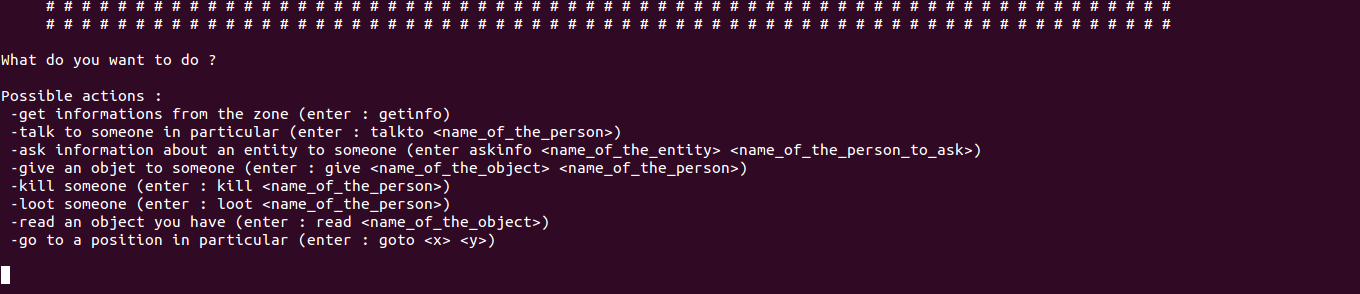
\includegraphics[width=1\textwidth]{images/screenshootUI01.png}
    \caption{Exemple d'action possibles}	
  \end{center}
\end{figure}

Si le joueur rentre autre chose qu'un des mot-clés prévus, cela provoque un message d'erreur. Les  execeptions et erreurs sont reportées à l'utilisateur. \\

Le jeu est actuellement en anglais, mais tous les messages d'interaction avec le joueur sont implémentés dans le code sous forme de constantes de façon à rendre le changement de langue le plus simple possible. Les mots clés sont sans rapport avec les noms des fonctions appelées derrière, il est donc egalement possible de les changer sans impacter le code.


  
\end{document}
